% !TeX root = ../../../../thesis.tex

\subsection{Modulator}

	The task of the modulator is to switch the LED on or off based on the ID that is assigned to the light fixture.
	It is the responsibility of this piece of hardware to translate the ID into the unique current signature.


	The way an LED (Light Emitting Diode) works, is that current has to flow through it in order for it to emit light.
	In other words, an LED is controlled via current, it is not controlled by applying a voltage to it.
	When a certain amount of current flows through the LED, a certain amount of voltage will drop over the LED.

	The easiest way to make an LED emit light, is to put a current limiting resistor in series with a voltage source and an LED.
	A schematic can be seen in \autoref{fig:dc-led-resistor}.
	But there exists no ideal DC power supply.
	Depending on the load, the provided voltage of the power supply may fluctuate.
	Due to the fluctuation of the provided voltage, the LED can start to change in brightness.
	The current that flows through the LED is a function of the voltage over the resistor and the value of the resistor: $I = \frac{U}{R}$.
	So if $U$, the provided voltage, is fluctuating, the current that flows through the LED, $I$, will also fluctuate.
	This causes the brightness of the LED to fluctuate.


	A better way to power an LED, is by using a current source.
	Where an ideal voltage source will always deliver a certain amount of voltage independent of the load, a current source will always deliver a certain amount of current independent of the load.
	If there will always be a constant amount of current flowing through the LED, the brightness will not fluctuate.
	In \autoref{fig:dc-led-current-source} a schematic can be seen, which shows an example of a current source powering an LED.
	This current source can be toggled on and off via a 0 V or 3.3/5 V signal, coming from a micro-controller, uC in the schematic.


	\begin{figure}[!h]
		\centering
		\begin{minipage}[b]{0.3\textwidth}
			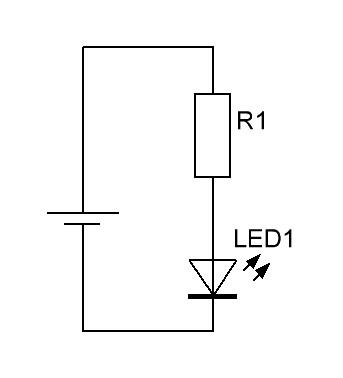
\includegraphics[width=\textwidth]{chapters/hardware-chapters/DC/dc-modulator/dc-led-resistor.jpg}
			\caption{Simplest way to power an LED.}
			\label{fig:dc-led-resistor}
		\end{minipage}
		\hfill
		\begin{minipage}[b]{0.5\textwidth}
			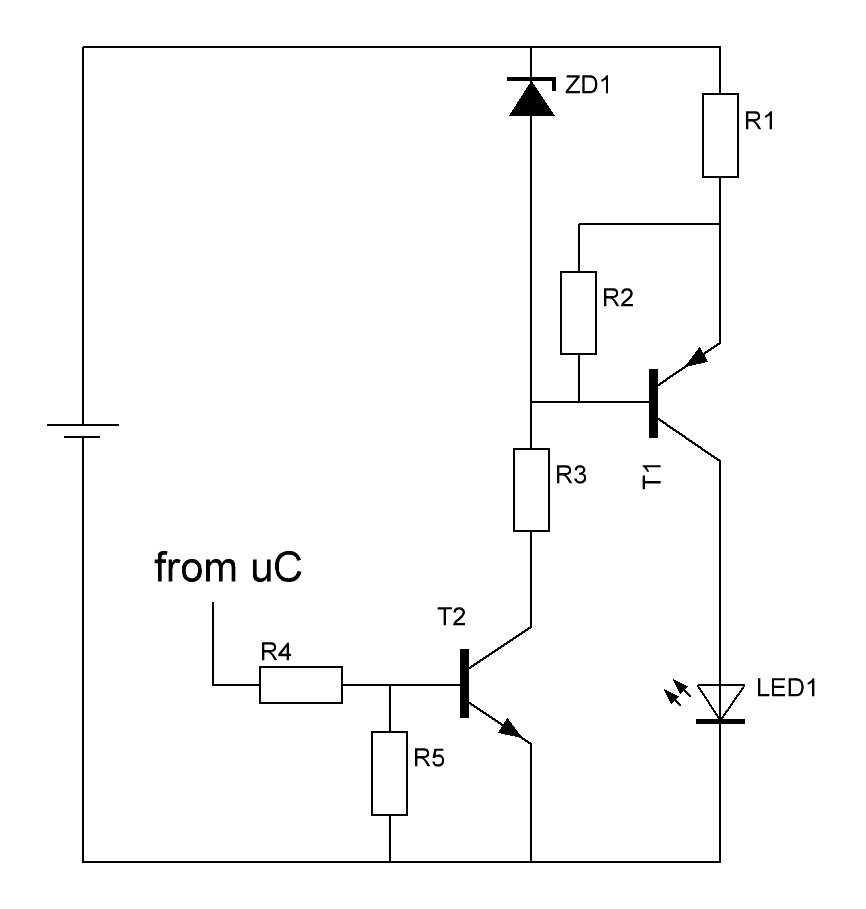
\includegraphics[width=\textwidth]{chapters/hardware-chapters/DC/dc-modulator/dc-led-current-source.jpg}
			\caption{Current source powering an LED.}
			\label{fig:dc-led-current-source}
		\end{minipage}
	\end{figure}

	By using a current source, two benefits can be identified:

	\begin{itemize}
		
		\item Since the current that flows through the LED is constant, the LED will not flicker.

		\item The current source will make sure that the current that is drawn, is either zero or some constant value depending on the bit that is being encoded.
		This will yield a signal with two distinct values.
		When multiple of these signals are aggregated and measured by a smart-meter, the measured signal will also have distinct values.
		This signal will make it easy to decode the information that was encoded by the modulators.

	\end{itemize}